%!TEX root = ../../thesis.tex

\section{Physics-Based Model} \label{sec:Physics_Based_Model}

In this section, we identify a difference equation for the temperature evolution using the Resistance-Capacitance (RC)  modeling method, via the Building Resistance-Capacitance Modeling (BRCM) MATLAB toolbox \cite{David}. 
To derive an RC building model, we first decompose the building into building elements (BE), such as the bulk volume of air in each room, walls, floors and ceilings. 
An electric analogy can then be used to obtain an equivalent electrical circuit whose resistances and capacitances represent thermal resistances and thermal capacitances of the BEs, and voltages and currents represent temperatures of BEs and heat transfers between those. 
With this equivalent electrical circuit in hand, the thermal dynamic model can be obtained by applying Ohm's law and Kirchhoff's circuit laws on this equivalent circuit.
The resulting building model is bilinear in nature, due to the physics of the HVAC system.
%The same dataset used to train the data-driven model in Section \ref{sec:Data_Driven_Model} is used to identify the physics-based model. 
%In this paper, we re-identify the building model using the same training dataset as used in Section \ref{sec:Data_Driven_Model}, and estimate distinct internal gains functions for different seasons.

%We derive a physics-based model using the Building Resistance-Capacitance Modeling (BRCM) MATLAB toolbox developed at ETH Zurich \cite{David}, which derives an RC model for a building using its geometry and construction data. 

%In brief, to derive an RC model, a building is decomposed into elements such as the bulk volume of air in each room, walls, floors and ceilings. An electrical analogy is then used to model these building elements using resistances and capacitances. For example, a capacitance can represent the thermal capacity of a wall and a resistance can represent the thermal resistance at the surface of a wall due to convection. In the analogous electrical circuit, voltages represent temperatures of different building elements and currents represent heat transfers between those. A main advantage of this approach is that the resulting model has a small number of parameters, even for a complex multi-zone building; furthermore, these parameters have strong physical meaning, which aids in their identification. 


%%%%%%%%%%%%%%%
\subsection{Model Setup}\label{sec:physics_model}

%Details of the derivation of the physics-based building model is described in \cite{Qie}. 
The physics-based building model has the following form \cite{Qie}:
\begin{subequations}\label{eq:physics_model}
\begin{align}
x(k+1) &= Ax(k)+B_v v(k) + B_\text{IG} f_\text{IG}(k) \label{eq:physics_model1} \\ \nonumber
	& \quad + \textstyle \sum_{i=1}^{21} \big( B_{xu_i} x(k) + B_{vu_i} v(k) \big) u_i(k) \label{eq:physics_model_2} \\
y(k) &= C x(k),
\end{align}
\end{subequations}
where the state vector $x \in \mathbb{R}^{289}$ represents temperatures of all building elements on the 4th floor and $y \in \mathbb{R}^6$ represents the average temperatures of the six zones shown in Figure \ref{fig:floor_plan}. $u \in \mathbb{R}^{21}$ denotes the airflow rate from the 21 VAV boxes, and $v := [v_\text{Ta}, v_\text{Ts}]^\top$ is the disturbance vector, which captures known disturbances from ambient air temperature and the HVAC system's supply air temperature. 
Note that from our previous studies, heat gains due to solar radiation are orders of magnitude less than those caused by other disturbances and inputs and hence are not included here. 
Finally, $f_\text{IG}(k) : \mathbb{N} \rightarrow \mathbb{R}^6$ captures internal gains in each of the six zones on the 4th floor. For week $m$ from the training set $\mathcal{T}$:
\begin{equation}\label{eq:fig}
f_\text{IG}(k) = f_\text{IG}^c + \begin{cases}
	f_{\text{IG},\mathcal{F}}^v(k), & ~\text{if} ~ m \in \mathcal{F}, \\
	f_{\text{IG},\mathcal{W}}^v(k), & ~\text{if} ~ m \in \mathcal{W}, \\
	f_{\text{IG},\mathcal{S}}^v(k), & ~\text{if} ~ m \in \mathcal{S}, \\
	\end{cases}
\end{equation}
where $f_\text{IG}^c$ is an unknown constant vector representing background heat gains due to idle appliances such as computers and printers. Functions $f_{\text{IG},\mathcal{F}}^v(\cdot)$, $f_{\text{IG},\mathcal{W}}^v(\cdot)$ and $f_{\text{IG},\mathcal{S}}^v(\cdot)$ are unknown nonparametric functions that capture the time-varying heat gain due to occupancy and equipments in fall, winter and spring, respectively.
The system matrices $A$, $B_v$, $B_\text{IG}$, $B_{xu_i}$ and $B_{vu_i}$ are functions of tuning parameters: the window heat transmission coefficient ($U_\text{win}$), the convection coefficients of the interior wall ($\gamma_\text{IW}$), the exterior wall ($\gamma_\text{EW}$), the floor ($\gamma_\text{floor}$), and the ceiling ($\gamma_\text{ceil}$). 
Define $\gamma := \begin{bmatrix} U_\text{win}, \gamma_\text{IW}, \gamma_\text{EW}, \gamma_\text{floor}, \gamma_\text{ceil}, f_\text{IG}^{c\top} \end{bmatrix}^\top \in \mathbb{R}^{11}$, then to identify the physics-based model, we need to estimate the parameter vector $\gamma$ as well as the functions $f_{\text{IG},\mathcal{X}}^v(\cdot),~\mathcal{X} \in \{\mathcal{F}, \mathcal{W}, \mathcal{S}\}$.
Next, we describe our approach for identifying this model.

%%%%%%%%%%%%%%%
\subsection{Model Identification}\label{sec:physics_id}

For a fair comparison, the same data used to train and test the data-driven model is used to train and validate the physics-based model. 
The model identification process is performed in two steps: First, the subset of the training data collected during weekends is used to estimate the parameters, $\gamma$. Second, the nonparametric functions $f_{\text{IG},\mathcal{X}}^v(\cdot)$ are estimated from the complete training dataset.

\vspace*{0.2cm}
\subsubsection{Parameter Estimation}
For parameter estimation purposes, we first set $f_{\text{IG},\mathcal{X}}^v(\cdot) = 0$ during the weekend days, and evaluate them at a later point (Equations (\ref{Eq:ig(k-1)})). With $f_{\text{IG},\mathcal{X}}^v(\cdot) = 0$, (\ref{eq:physics_model}) reduces to a purely parametric model:
\begin{equation}\label{eq:physics_parammodel}
\begin{aligned}
x(k+1) &= Ax(k)+B_v v(k) + B_\text{IG} f_\text{IG}^c\\
	& \quad + \textstyle \sum_{i=1}^{21} \big( B_{xu_i} x(k) + B_{vu_i} v(k) \big) u_i(k), \\
y(k) &= C x(k).
\end{aligned}
\end{equation}
The optimal model parameters are estimated by solving the following optimization problem:
\begin{equation}\label{eq:physics_opt}
\begin{aligned}
 \hat{\gamma} =&~\arg\min_{\gamma > 0}~\textstyle \sum_{m \in \mathcal{T}} \sum_k \Vert y_m(k,\gamma) - \bar y_m(k) \Vert ^ 2 \\
\text{s.t.~~}
&y_m(k,\gamma) \text{~and~} x_m(k,\gamma) \text{~satisfy (\ref{eq:physics_parammodel}) with}\\
&x_m(0) = x_{\text{KF},m}(0)\\
&u_m(k) = \bar u_m(k), v_m(k) = \bar v_m(k)~\forall~k,\\
\end{aligned}
\end{equation}

%\begin{equation}\label{eq:physics_opt}
%\begin{aligned}
% \hat{\gamma} =&~\arg\min_{\gamma > 0}~\left(J_\text{f} + J_\text{w} + J_\text{s} \right) \\
%\text{s.t.~~}
%&J_m = \textstyle \sum_k \Vert y_m(k,\gamma) - \bar y_m(k) \Vert ^ 2 ~ \text{for} ~ m \in \lbrace \text{f}, \text{w}, \text{s} \rbrace\\
%%&\text{where $y_m(k,\gamma)$ and $x_m(k,\gamma)$ satisfy (\ref{eq:physics_parammodel})} \\
%&y_m(k,\gamma) \text{~and~} x_m(k,\gamma) \text{~satisfy (\ref{eq:physics_parammodel}) with}\\
%&x_m(0) = x_{\text{KF},m}(0)\\
%&u_m(k) = \bar u_m(k), v_m(k) = \bar v_m(k)~\forall~k,\\
%\end{aligned}
%\end{equation}
\noindent
where $\bar u$, $\bar v$ and $\bar y$ denote the measured inputs, disturbances, and zone temperatures, respectively. In other words, we choose $\gamma$ such that, when the model is simulated with this set of parameter values and the measured inputs and disturbances, the sum of squared errors between the measured zone temperatures and the simulated temperatures is minimized.
The initial state $x_m(0)$ is required to simulate the model, however, not all states are measurable (the wall temperature for example is not), thus we estimate the initial states using a Kalman Filter $x_{\text{KF},m}(0)$, and set  $x_m(0) = x_{\text{KF},m}(0)$.
Furthermore, to compensate for the lack of sufficient excitation of the building, initial guesses for $\gamma$ that are physically plausible are chosen. The optimal parameter values are similar to those reported in \cite{Qie} and hence are not included here due to space limitations.
%The optimal parameter values are reported in Table \ref{table:param}.

%\begin{table}
%	\centering
%	\begin{tabular}{l l l}
%	\hline
%	Parameter & Description & Value [Unit]\\
%	\hline
%	$\gamma_{\text{EW}}$ & Exterior Wall Convection Coeff. & 50.0  [W/(m$^2$K)]\\
%	$\gamma_{\text{IW}}$ & Interior Wall Convection Coeff. & 12.8  [W/(m$^2$K)]\\
%	$\gamma_{\text{floor}}$ & Floor Convection Coeff. & 50.0  [W/(m$^2$K)]\\
%	$\gamma_{\text{ceil}}$ & Ceiling Convection Coeff. & 5.0  [W/(m$^2$K)]\\
%	$U_{\text{win}}$ & Window Heat Transmission Coeff. & 5.5  [W/(m$^2$K)]\\
%	$f^c_{\text{IG,NW}}$ & Background Heat Gain in Zone NW  & 25.6  [W/m$^2$]\\
%	$f^c_{\text{IG,W}}$ & Background Heat Gain in Zone W  & 20.6  [W/m$^2$]\\
%	$f^c_{\text{IG,S}}$ & Background Heat Gain in Zone S  & 15.9  [W/m$^2$]\\
%	$f^c_{\text{IG,E}}$ & Background Heat Gain in Zone E  & 16.4  [W/m$^2$]\\
%	$f^c_{\text{IG,NE}}$ & Background Heat Gain in Zone NE  & 19.9  [W/m$^2$]\\
%	$f^c_{\text{IG,C}}$ & Background Heat Gain in Zone C  & 6.8  [W/m$^2$]\\			
%	\hline
%	\end{tabular}
%	\caption{List of Model Parameters}
%	\label{table:param}
%\end{table}

%%%%%%%%%
\vspace*{0.2cm}
\subsubsection{Estimation of $f_\text{IG}^v(\cdot)$ for Each Season}
%After that, we use the entire training data for each season to estimate the occupancy function $f(\cdot)$. 
Let $f_{\text{IG},m}^v(\cdot)$, $m \in \mathcal{T}$ be an instance of the internal gains function $f_{\text{IG}}^v(\cdot)$ estimated for week $m$ in the training set. 
The optimal estimate for a given season, say fall, is then defined as the the average of all estimates for that season:
\begin{equation}
\hat {f}_{\text{IG},\mathcal{F}}^v(k) = \textstyle \sum_{m \in \mathcal{F}} f^v_{\text{IG},m}(k) / \| \mathcal{F} \| \quad \forall~k,
\end{equation}
where $\| \mathcal{F} \| $ represents the cardinality of set $\mathcal{F}$.
%Let $f_{\text{IG},\mathcal{X},w}^v(\cdot)$ be an instance of the internal gains function $f_{\text{IG},\mathcal{X}}^v(\cdot)$ estimated for week $w$ in season $\mathcal{X}$, where $\mathcal{X} \in \{\mathcal{F}, \mathcal{W}, \mathcal{S}\}$. 
%Let $\mathcal{W}_m = \{1,2,\ldots,n_m\}$ denote the set of weeks in the training data for season $m$, and let $f_{\text{IG},m,w}^v(\cdot)$ be an instance of the internal gains function $f_{\text{IG},m}^v(\cdot)$ estimated for week $w$ in $\mathcal{W}_m$. 
%The optimal $\hat {f}_{\text{IG},\mathcal{X}}^v(\cdot)$ is defined as the average of all estimates for a given season. 

To estimate $f_{\text{IG},m}^v(\cdot)$ for a given week $m$, let $\tilde x(k)$ and $\tilde{y}(k)$ denote the predicted states and zone temperatures at time $k$, with $f_{\text{IG},w}^v(k-1) = 0$, i.e.,
\begin{equation}\label{Eq:xnoig_ynoig}
	\begin{aligned}
	\tilde x(k) & = Ax(k-1)+B_v v(k-1) + B_\text{IG} f^c_\text{IG} \\
		& \quad + \textstyle \sum_{i=1}^{21} \big( B_{xu_i} x(k-1) + B_{vu_i} v(k-1) \big) \\
		& \quad \cdot u_{i}(k-1), \\
	\tilde y & = C \tilde x(k).
	\end{aligned}
\end{equation} 
By noting $x(k) = \tilde{x}(k) + B_\text{IG} f^v_{\text{IG},m}(k-1)$, $f^v_{\text{IG},m}(k-1)$ can be estimated by solving the following set of linear equations using Ordinary Least Squares:
\begin{equation}\label{Eq:ig(k-1)}
(C B_\text{IG}) \cdot f_{\text{IG},m}^v(k-1) = \bar{y}(k) - \tilde{y}(k),
\end{equation}
where $\bar{y}(k)$ is the measured zone temperatures at time $k$.  
%Finally, $\hat {f}_{\text{IG},m}^v(\cdot)$ is chosen as the average of all the estimates:
%\begin{equation}\label{Eq:fixed_ig}
%\hat {f}_{\text{IG},m}^v(k) = \frac{ \textstyle \sum_{w=1}^{n_m} f^v_{\text{IG},m,w}(k)}{n_m} \quad \forall~k.
%\end{equation}
%Therefore, the estimated function $\hat {f}_{\text{IG},m}^v(\cdot)$ takes into account the effect of hour of the day and day of the week on the internal gains.

%More specifically, let $\tilde x_w(k)$ and $\tilde{y}_w(k)$ denote the predicted states and zone temperatures at time $k$, with $f_{\text{IG},m,w}^v(k-1) = 0$, i.e.,
%\begin{equation}\label{Eq:xnoig_ynoig}
%	\begin{aligned}
%	\tilde x_w(k) & = Ax_w(k-1)+B_v v_w(k-1) + B_\text{IG} f^c_\text{IG} \\
%		& \quad + \textstyle \sum_{i=1}^{21} \big( B_{xu_i} x_w(k-1) + B_{vu_i} v_w(k-1) \big) \\
%		& \quad \cdot u_{w,i}(k-1), \\
%	\tilde y_w & = C \tilde x_w(k).
%	\end{aligned}
%\end{equation} 
%By noting $x_w(k) = \tilde{x}_w(k) + B_\text{IG} f^v_{\text{IG},m,w}(k-1)$, we can estimate $f^v_{\text{IG},m,w}(k-1)$ by solving the following set of linear equations using Ordinary Least Squares:
%\begin{equation}\label{Eq:ig(k-1)}
%(C B_\text{IG}) \cdot f_{\text{IG},m,w}^v(k-1) = \bar{y}_w(k) - \tilde{y}_w(k),
%\end{equation}
%where $\bar{y}_w(k)$ represents measured zone temperatures at time $k$.  
%Finally, $\hat {f}_{\text{IG},m}^v(\cdot)$ is chosen as the average of all the estimates:
%\begin{equation}\label{Eq:fixed_ig}
%\hat {f}_{\text{IG},m}^v(k) = \frac{ \textstyle \sum_{w=1}^{n_m} f^v_{\text{IG},m,w}(k)}{n_m} \quad \forall~k.
%\end{equation}
%Therefore, the estimated function $\hat {f}_{\text{IG},m}^v(\cdot)$ takes into account the effect of hour of the day and day of the week on the internal gains.

%%%%%%%%%%%%%%%
\subsection{Results}\label{sec:physics_results}

The identified model is tested on holdout test weeks from different seasons. The average daily prediction RMS errors by zone and season are reported in Table \ref{tab:data_RMS_zones}. Figure \ref{fig:physics_qig} shows the estimated increase in zone temperatures due to internal gains for fall, winter and spring. %: $B_\text{IG}\cdot \big( f^c_\text{IG} + f^v_{\text{IG},m}(k) \big)$ for $m \in$ \{f, w, s\}, respectively. 
Similar average internal gains are observed for all zones and seasons. The zones that correspond to open workspaces and conference rooms (``West'', ``South'', ``East'' and ``Center'') show discernible daily peaks in their internal gains profiles with a slight decrease during weekends. Furthermore, there is little variation in the internal gains profiles across different seasons.
\begin{figure}
	\centering
	\vspace*{-0.3cm}
	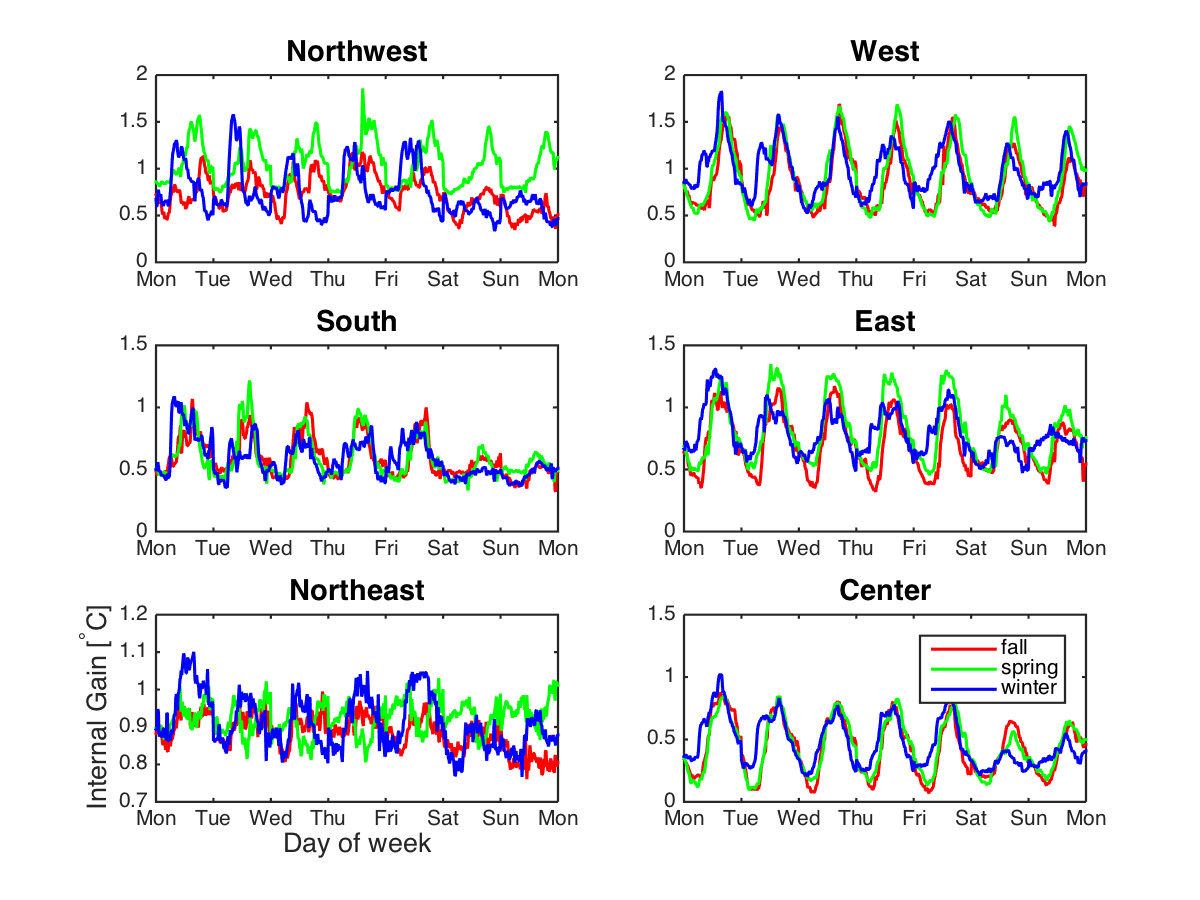
\includegraphics[width=\textwidth]{chapters/building_model/figures/physics_qig.png}
	\vspace*{-0.2cm}
	\caption{Estimated Internal Gain $f_{\text{IG}}$ from the Physics-Based Model by Zone and Season}
	\vspace*{-0.5cm}
	\label{fig:physics_qig}
\end{figure}